%#!platex -kanji=utf8 hb.tex
\chapter{書体}
% これはただのダミーテキスト.
% 文字コードを判定するための意味のない文字列.
% これくらい記述すれば大丈夫かな.
% Emacs のくせに生意気な.
% Emacs の分際で自動判別とか.
% Mac OS X のテキストエディッタの文字コード自動判別はうまくいかないぞ.

%\section{書体の高さとライン}
%
%\mada{\TeX/\LaTeX との関係と説明を追加}
%
%\begin{figure}[htbp]
% \centering
% 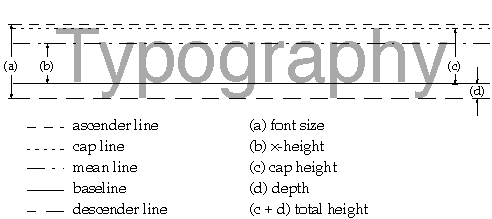
\includegraphics{typeface-lines}
% \caption{書体の高さとライン}\figlab{書体の高さとライン}
%\end{figure}

\section{文章の強調}

\subsection{欧文の文字列を強調する}
\CI{emph}%
\begin{usage}
\emph{$\<強調したい文字列>$} 
\end{usage}
\begin{inout}
``The \emph{\TeX book} has good examples, 
 problems and jokes.''
\end{inout}

\subsection{日本語の文字列を強調する}
\CI{emph}%
\begingroup
 \let \origcmd = \emph
 \def \emph#1{\origcmd{{\gtfamily\bfseries#1}}}%
\begin{usage}
\emph{$\<強調したい文字列>$}  
\end{usage}
\begin{inout}
 環境とインタラクションするエージェントが,現在の状態を観測し,
 次状態で振る舞うべき行動を選択するための教師なし学習としては
 \emph{強化学習}が知られている.
\end{inout}
\endgroup

%場合によっては \Cmd{em} コマンドが使えます.これは
%\KY{宣言型コマンド}\pp{\secref{ml:command}}と
%呼ばれるもので,広範囲な論理強調に使う事ができます.
%ただしこのコマンドを使うならば\KY{イタリック補正}を
%挿入する場合があります.イタリック補正とはイタリック体の
%文字の直後にローマン体などの別のフォントが来た場合に
%挿入すべき空白の事です.{\LaTeX}が用意している \Cmd{emph} 
%や \Cmd{textit}などはこのイタリック補正
%が適切に挿入されるようになっています.宣言型の強
%調コマンド \Cmd{em}を使う場合は%
%\glossary{"/@\hspace*{-1.2ex}\verb+"\/+}%"
%自分で挿入しますから \cmd{/} 命令を使う事になります.%"
%\begin{inout}
%\emph{Future University-Hakodate} 
%is interesting.\par 
%{\em FUN\/} is funky?\par
%{\em FUN} is not funky?
%\end{inout}



\section{文字の大きさ}\seclab{font}

%\KY{文字} (\Z{character}) は\Z{意思伝達手段}であって,
%長いあいだに洗練された\Z{媒体}です.怒りの意思を強く込
%めたいならば人は荒々しく文字を書くでしょうし,優しさを
%込めたいならば丸みを帯びた書き方になるでしょう.以上の
%ような文字の形を\KY{書体} (\Z{typeface}) と呼びます.
%
%世の中ではこれらを書体というひとつの枠組みで整理してい
%ます.書体は読者に対して何らかのメッセージを分かりやす
%く伝えるために変更される場合があります.ですから書体を
%変更するという事には必ず意味があるべきなのです.むや
%みやたらに書体を変更しても逆に読者を混乱させます.また
%自分だけのルールで書体を変更しても読者には何の意味なの
%かが分かりませんので,一般的に使われている書体に関する
%ルールを守るのもマナーです.

%{\LaTeX}は\Z{マークアップ}型のシステムなのでユーザが
%直接書体変更用の命令を使う事は本来ならば必要のない事
%だと思われます.以下のコマンドは直接使うのではなく新
%規に環境を定義して用いるのが望ましいでしょう.

\subsection{文字を大きくする}
\CIS{large,Large,LARGE,huge,Huge}%
\begin{usage}
{\large $\<やや大きくしたい文字列>$}
{\Large $\<大きくしたい文字列>$}
{\LARGE $\<かなり大きくしたい文字列>$}
{\huge $\<とても大きくしたい文字列>$} 
{\Huge $\<特大にしたい文字列>$}
\end{usage}

\begin{inout}
{\large やや大きい}  {\Large 大きい} {\LARGE かなり大きい}
{\huge とても大きい} {\Huge 特大}
\end{inout}

\subsection{文字を小さくする}
\CIS{tiny,scriptsize,footnotesize,small}
\begin{usage}
{\small $\<やや小さくしたい文字列>$}
{\footnotesize $\<小さくしたい文字列>$}
{\scriptsize $\<かなり小さくしたい文字列>$}
{\tiny $\<とても小さくしたい文字列>$}
\end{usage}

\begin{inout}
{\small やや小さい}        {\footnotesize 小さい}
{\scriptsize かなり小さい} {\tiny とても小さい}
\end{inout}

\subsection{文字を通常の大きさにする}
\CI{normalsize}
\begin{usage}
{\normalsize $\<通常の大きさに戻す文字列>$} 
\end{usage}

\begin{inout}
{\small この部分は小さいですが,{\normalsize この部分は
 通常の大きさの文字列}になります.}
\end{inout}


\section{文章の一部の書体を変更する}\seclab{ouyou:font}
\index{ローマン体}%
\index{サンセリフ体}%
\index{タイプライタ体}%
\index{ミディアム体}%
\index{ボールド体}%
\index{イタリック体}%
\index{スラント体}%
\index{スモールキャピタル体}%

\subsection{ファミリーを変更する}
\CIS{rmfamily,sffamily,ttfamily,textrm,textsf,texttt}
\begin{usage}
{\rmfamily $\<ローマン>$}     \textrm{$\<ローマン>$}
{\sffamily $\<サンセリフ>$}   \textsf{$\<サンセリフ>$}
{\ttfamily $\<タイプライタ>$} \texttt{$\<タイプライタ>$}
\end{usage}

\begin{inout}
{\sffamily This is sans serif family font}. 
However \texttt{this is typewriter family font}.
\end{inout}

\subsection{シリーズを変更する}
\CIS{mdseries,textmd,bfseries,textbf}
\begin{usage}
{\mdseries $\<ミディアム>$} \textmd{$\<ミディアム>$}
{\bfseries $\<ボールド>$}   \textbf{$\<ボールド>$}
\end{usage}

\begin{inout}
Would you \textbf{pass} me the salt?
OK.\@ Here you are.
\end{inout}

\subsection{シェイプを変更する}
\CIS{itshape,slshape,scshape,textit,textsl,textsc}
\begin{usage}
{\itshape $\<イタリック>$} \textit{$\<イタリック>$} 
{\slshape $\<スラント>$} \textsl{$\<スラント>$}
{\scshape $\<スモールキャップ>$} \textsc{$\<スモールキャップ>$}
\end{usage}

\begin{inout}
We can accept \textsc{Html}, \textsc{Pdf}, and 
 {\slshape PostScript} format files.
\end{inout}

\subsection{ファミリ,シリーズ,シェイプ,サイズを同時に変更する}
\begin{usage}
{$\<サイズ>$ $\<ファミリ>$ $\<シリーズ>$ $\<シェイプ>$ $\<文字列>$} 
\end{usage}

\begin{inout}
\textsf{\textbf{Sans serif bold typeface}} and 
 {\sffamily\bfseries same typeface}
\end{inout}

\subsection{和文の書体を変更する}
\CIS{gtfamily,textgt,textmc,mcfamily}%
\begin{usage}
{\gffamily $\<ゴシック>$} \textgt{$\<ゴシック>$}
{\mcfamily $\<明朝>$}     \textmc{$\<明朝>$}
\end{usage}

\begin{inout}
 和文組版において明朝体は通常の文章の組版,ゴシック体は
\textgt{文章の強調に}使われます.{\gtfamily 見出しも強
調すべき要素なのでゴシック体にするのが普通です}. 
\end{inout}

\section{文章の書体を変更する}


\begin{table}[htbp]
 \begin{center} \footnotesize
  \caption{フォント関連のパッケージ一覧}\tablab{fontpac}
  \begin{tabular}{llllll} 
   \TR
   \Th{パッケージ}  & \Th{ローマン体}   & \Th{サンセリフ体}   & \Th{タイ
   プライタ体} 
    & \Th{数式}\\
   \MR
   % European Computer Modern: cm-super ec tc tt2001
   % European Modern: EM (PS)
   % Latin Modern LM (PS)
   % cm blue sky (PS), cm bakoma (PS, trutype), cm (Metafont)
   % ↑ここまで突っ込まない.
   指定なし    & CM~Roman & CM~Sans~Serif & CM~Typewriter & CM~Roman\\
   \hline
   \Y{lmodern} & LM~Roman & LM~Sans~Serif & LM~Typewriter & \\
   % Latin modern fonts in type 1 format based on the Computer Modern fonts
   % ただし,\usepackage[T1]{fontenc}必要
   \Y{type1cm} & CM~Roman & CM~Sans~Serif & CM~Typewriter & \\
   % ただし,\usepackage[T1]{fontenc}の時は type1ec 互換
   \Y{type1ec} & EC~Roman & EC~Sans~Serif & EC~Typewriter & \\
   % Computer modern fonts in T1 and TS1 encodings.
   \hline
   \Y{txfonts} & Times風    & Helvetica風  & Monospaced風   & Times風\\
   \Y{pxfonts} & Palatino風 & Helvetica風  & Monospaced風   & Palatino風\\
   \hline
   \Y{mathptmx}& Times      &              &                & Times \\
   \Y{mathpazo}& Palatino   &              &                & Palatino\\
   \hline
   \Y{bookman} & Bookman    & Avant Garde  & Courier        & \\
   \Y{newcent} & New~Century & Avant Garde & Courier & \\[-2pt]
               &  Schoolbook\\
   \Y{helvet}  &            & Helvetica    &                & \\
   \Y{avant}   &            & Avant Garde  &                & \\
   \Y{courier} &            &              & Courier        & \\
   \hline
   \Y{charter} & Charter    &              &                & \\
   \Y{chancery}& Zapf &           &                & \\[-2pt]
               & Chancery\\
%   \Y{pifont}  & & & \\
%   \Y{mathptm} & Times & &  & Times\\%obsolete
%   \Y{mathppl} & Palatino & &  & Palatino\\%obsolete
%   \Y{times}   & Times      & Helvetica    & Courier        & \\%obsolete
%   \Y{palatino}& Palatino   & Helvetica    & Courier        & \\%obsolete
   \BR
  \end{tabular}
 \end{center}
\end{table}

\subsection{文字の書体を変更する}

\begin{inonly}
\usepackage{lmodern} 
\end{inonly}
\fontsmpl{lmr}{lmss}{lmtt}

\begin{inonly}
\usepackage{txfonts} 
\end{inonly}
\fontsmpl{txr}{txss}{txtt}

\begin{inonly}
\usepackage{pxfonts} 
\end{inonly}
\fontsmpl{pxr}{pxss}{pxtt}

\begin{inonly}
\usepackage{bookman}
\end{inonly}
\fontsmpl{pbk}{pag}{pcr}

\begin{inonly}
\usepackage{newcent} 
\end{inonly}
\fontsmpl{pnc}{pag}{pcr}


\begin{inonly}
\usepackage{helvet} 
\end{inonly}
\fontsmplone{T1}{phv}{m}{n}

\begin{inonly}
\usepackage{avant} % Avant Garde
\end{inonly}
\fontsmplone{T1}{pag}{m}{n}

\begin{inonly}
\usepackage{courier} 
\end{inonly}
\fontsmplone{T1}{pcr}{m}{n}

\begin{inonly}
\usepackage{charter} 
\end{inonly}
\fontsmplone{T1}{bch}{m}{n}

\begin{inonly}
\usepackage{chancery} 
\end{inonly}
\fontsmplone{T1}{pzc}{m}{n}

%\begin{intext}
%\usepackage[scaled]{helvet}
%\end{intext}

%\begin{intext}
%\usepackage[T1]{fontenc}
%\usepackage{textcomp}
%\usepackage{type1ec}
%\end{intext}

%\Y{fontenc}パッケージと\Y{textcomp}は\kenten{おまじない}的に
%記述した方が良いでしょう.

%\begin{Exe}
%a既存の原稿に以下の記述を追加し,タイプセットの実行結果を吟味してください.

%\begin{intext}
%\usepackge[T1]{fontenc}
%\usepackage{textcomp}
%\usepackage{type1ec}
%\end{intext}

%また,`\verb|\usepackage{type1ec}|'となっている箇所を,
%\Y{type1cm}, \Y{lmodern}, \Y{txfonts}, \Y{pxfonts}
%等でも試してみてください.
%\end{Exe}


\subsection{Timesと比較してHelveticaを少し縮小する}
\Y{helvet}は \Z{Times} 等に比べて若干大きいので,\option{scaled}オプションで
拡大縮小すると良いでしょう.

\begin{intext}
\usepackage[scaled=.92]{helvet}
\end{intext}

単に \Option{scaled} オプションだけを記述した場合は 0.95 倍されます.

\begin{intext}
\usepackage[scaled]{helvet} % 標準は 0.95 倍
\end{intext}




\subsection{Palatino, Helvetica, Courierを使う}
%\begin{Prob}
%\Z{Palatino}, Helvetica, Courierを基本的に用いるよう
%な設定は次のようになります.実際にタイプセットし,その出力結果を吟味してく
%ださい.

\begin{inonly}
\usepackage{mathpazo}% palatino
\usepackage[scaled]{helvet}% Helvetica
\usepackage{courier}% Courier
\end{inonly} 
\fontsmpl{ppl}{phv}{pcr}% pplj?


\subsection{Times, Helvetica, Courierを使う}
%Times, Helvetica, Courierを基本的に用いるようにする設定は
%次のようになります.
\begin{inonly}
\usepackage{mathptmx}% Times
\usepackage[scaled]{helvet}% Helvetica
\usepackage{courier}% Courier
\end{inonly}
\fontsmpl{ptm}{phv}{pcr}% pplj?

%この設定と \Y{txfonts} パッケージを使った場合の出力は
%どのように異なるのか,実際にタイプセットして確認してみてください.

% mathptm では mathcal に Zapf Chancery が使われていた,
% AMSFonts の eucal はこの古いものを使えるようになっている.
% psamsfonts オプションを使うとフリーの Type 1 フォントだけを
% 使うように設定される.
%\end{Prob}

%mathpple.sty
%mathptm
%mathptmx

%\YI{utopia}
%\begin{inonly}
%\usepackage{utopia} 
%\end{inonly}
%\fontsmpl{put}{cmss}{cmtt}
%\begin{figure}[htbp]
% \begin{center}
\newcommand*\mathimage[2][clip]{%
  \noindent%\hbox{%
    {\includegraphics[#1]{mathFontTest/smpl-#2-crop}}%\space
    %{\sty{#2}}%
  %}\par%
}%
%
% \caption{基本書体の変更例}\figlab{basic:font:change}
% \end{center}
%\end{figure}

\section{数式書体を変更する}

\subsection{\Y{type1cm}を使う}
\begin{inonly}
\usepackage{tyep1cm}
\end{inonly}
\begin{outonly}
\mathimage[bb=0 0 189 95]{type1cm}% 
\end{outonly}

\subsection{\Y{euler}を使う}
\begin{inonly}
\usepackage{euler} 
\end{inonly}
\begin{outonly}
\mathimage[bb=0 0 190 95]{euler}%
\end{outonly}

\clearpage

\subsection{\Y{mathpazo}を使う}
\begin{inonly}
\usepackage{mathpazo} 
\end{inonly}
\begin{outonly}
\mathimage[bb=0 0 187 88]{mathpazo}% 
\end{outonly}

\subsection{\Y{pxfonts}を使う}
\begin{inonly}
\usepackage{pxfonts}  
\end{inonly}
\begin{outonly}
\mathimage[bb=0 0 173 96]{pxfonts}% 
\end{outonly}

\clearpage

\subsection{\Y{mathptmx}を使う}
\begin{inonly}
\usepackage{mathptmx}  
\end{inonly}
\begin{outonly}
\mathimage[bb=0 0 169 86]{mathptmx}%
\end{outonly}

\subsection{\Y{txfonts}を使う}
\begin{inonly}
\usepackage{txfonts}  
\end{inonly}
\begin{outonly}
\mathimage[bb=0 0 166 93]{txfonts}% 
\end{outonly}

%\usepackage{concmath}
%\usepackage{concrete}
%\usepackage{cmbright}

